\chapter{Selection of Dynamical Reputation Model parameters}
\label{App:parameters}

The Dynamical Reputation Model(DIBRM) has several tuning parameters. In previous studies the model \cite{melnikov2018toward,yashkina2020} was used to approximate real reputation on Stack Exchange sites \cite{yashkina2020}, so model parameters were $t_a =2, \beta = 1, \alpha = 1.4$, while the basic reputation value $I_{bn}$ was +2 or +4. As $\beta=1$, the forgetting factor is not considered. Our goal was to describe how reputation influences the sustainability of the community. Further, we wanted to resemble the concept of trust. Our tuning procedure differs than in previous studies on Stack Exchange sites, and we ended up with different model parameters. 

For \textbf{basic reputation} contribution we selected $I_{bn}=1$. With this values each interaction has initial contribution $+1$. 

For \textbf{characteristic time} $t_a$ we choose $t_a=1$. The median/average time between subsequent interactions is $1 day$. If time window between two interactions is less than $1 day$ they reputation will rise, otherwise, the reputation decays.

\begin{figure}[h]
	\centering
	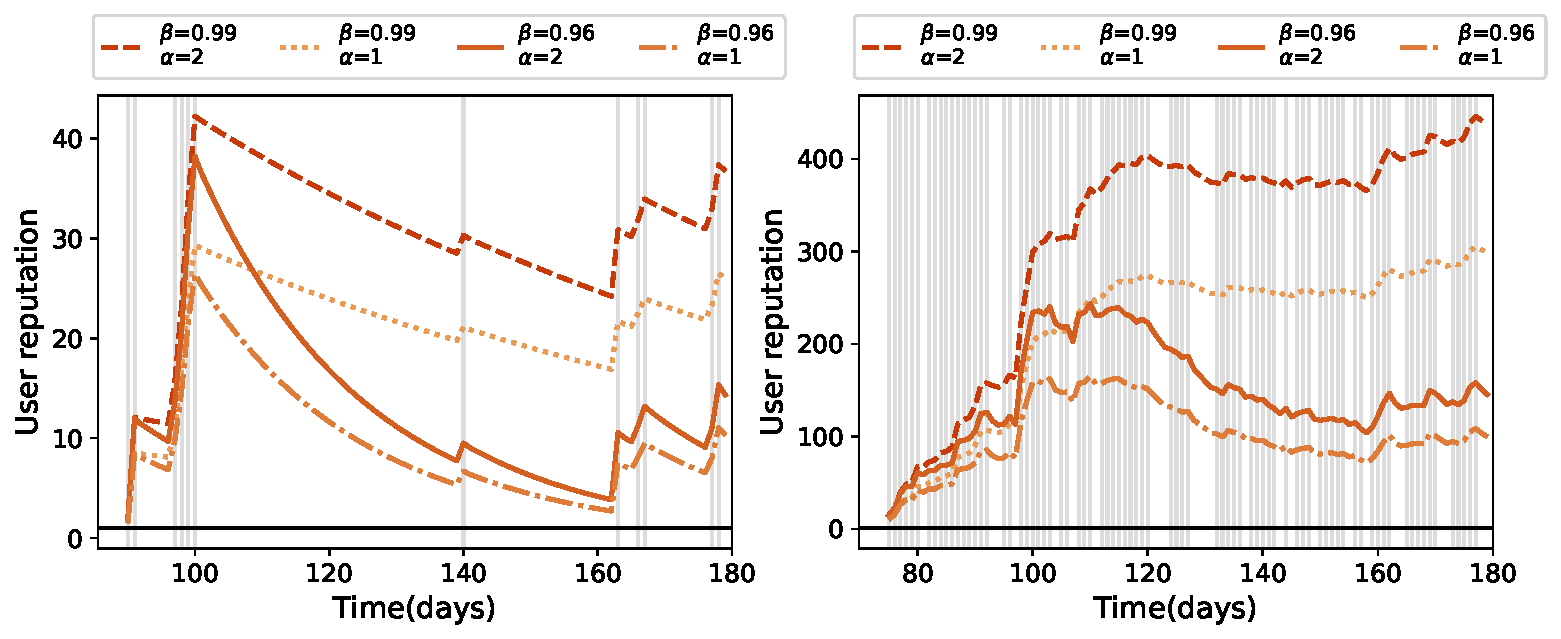
\includegraphics[width=0.8\linewidth]{figures/stackexchange/single_user_reputation.pdf}
	\caption[Single users reputations.]{Single users reputations }
	\label{fig:singleuser}
\end{figure} 

The {parameter $\alpha$} represents the \textbf{cumulative factor}. The burst in activity and recent interactions lead to higher reputation values with larger parameter $\alpha$. The figure \ref{fig:singleuser} represents reputations of two selected users from SE. The first one is sporadically active, while the second one makes frequent interactions. We calculate the reputation of these two users for different parameters $(\alpha, \beta)$. We selected $\alpha=2$.  

The reputation decay determines the \textbf{forgetting factor $\beta$}. We set parameter on $\beta=0.96$. The reputation should reflect properties of the trust. This means that we do not expect to $\beta$ be high, as then inactive users keep larger reputation values. In figure \ref{fig:singleuser} for $\beta=0.99$ even for little active user reputation stays higher during observed period. With lower $\beta$ it may drop to the reputation threshold and indicate that user stoped to be active.  

We compared the number of users with estimated reputation higher than 1 for different parameters $\beta$ and concluded that $\beta$ close to $0.96$ approximates the number of users with recorded interactions in a given 30 days sliding window. For each pair of communities we calculated number of users with at least one interactions in every 30 days sliding window and then we estimated several times series expressing the number of users with reputation higher than 1 for fixed $\beta$. Then we calculated the root mean square error (RMSE) between those time series for the first 200 days. Values of RMSE are shown on Figure~\ref{fig:rmse}. For each community, we can find parameter $\beta$ that minimizes RMSE. Although $\beta$ does not have a unique value across communities, it varies between 0.95 and 0.96.  

\begin{figure}[h!]
	\centering
	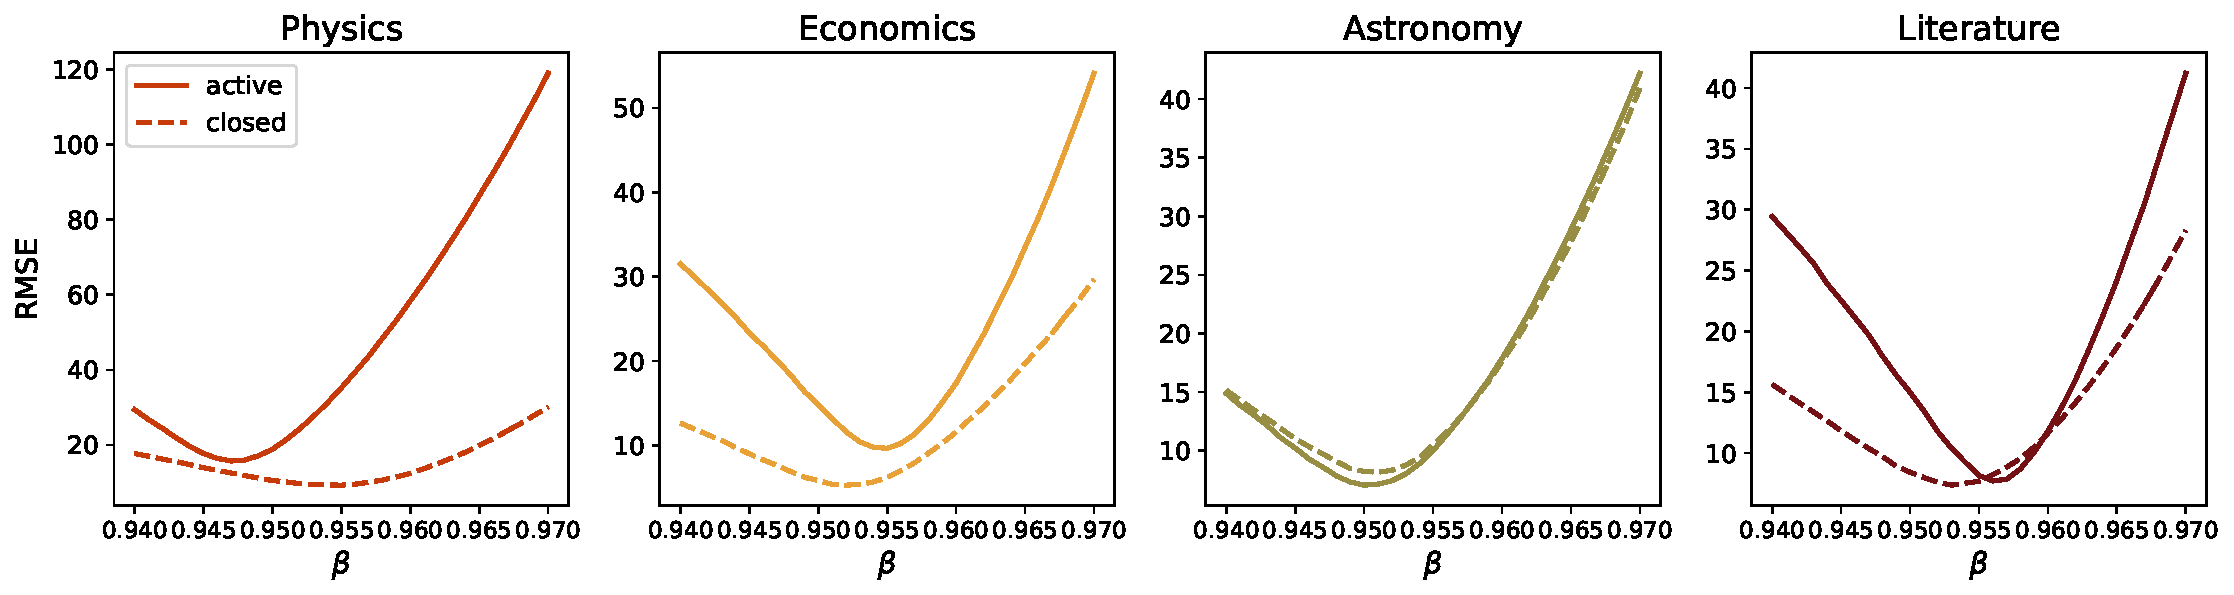
\includegraphics[width=\linewidth]{figures/stackexchange/rmse.pdf}
	\caption[RMSE between number of users in 30 days sliding window and positive reputation.]{RMSE between number of active users in sliding window of 30 days and number of users with reputation $>1$ for  $0.94< \beta <0.97$ with step $0.001$. }
	\label{fig:rmse}
\end{figure}

Figure \ref{fig:nusers} shows comparison between number of users in 30 days sliding window, number of users for these optimal values $\beta = 0.954$ and $\beta =0.96$. For $\beta = 0.96$ we observe that in most communities estimated number of active users consistently slightly higher than the actual number of users which have made at least one interaction in that sliding window. This means that dynamic reputation model in some cases overestimates the reputation of the user, but far more important is that it never understimates the real number of active users. Since we base our calculations of total and average reputation within the community only on users whose reputation is higher than the threshold this is important as no active users are disregarded by the model due to the value of the decay parameter.

\begin{figure}[H]
	\centering
	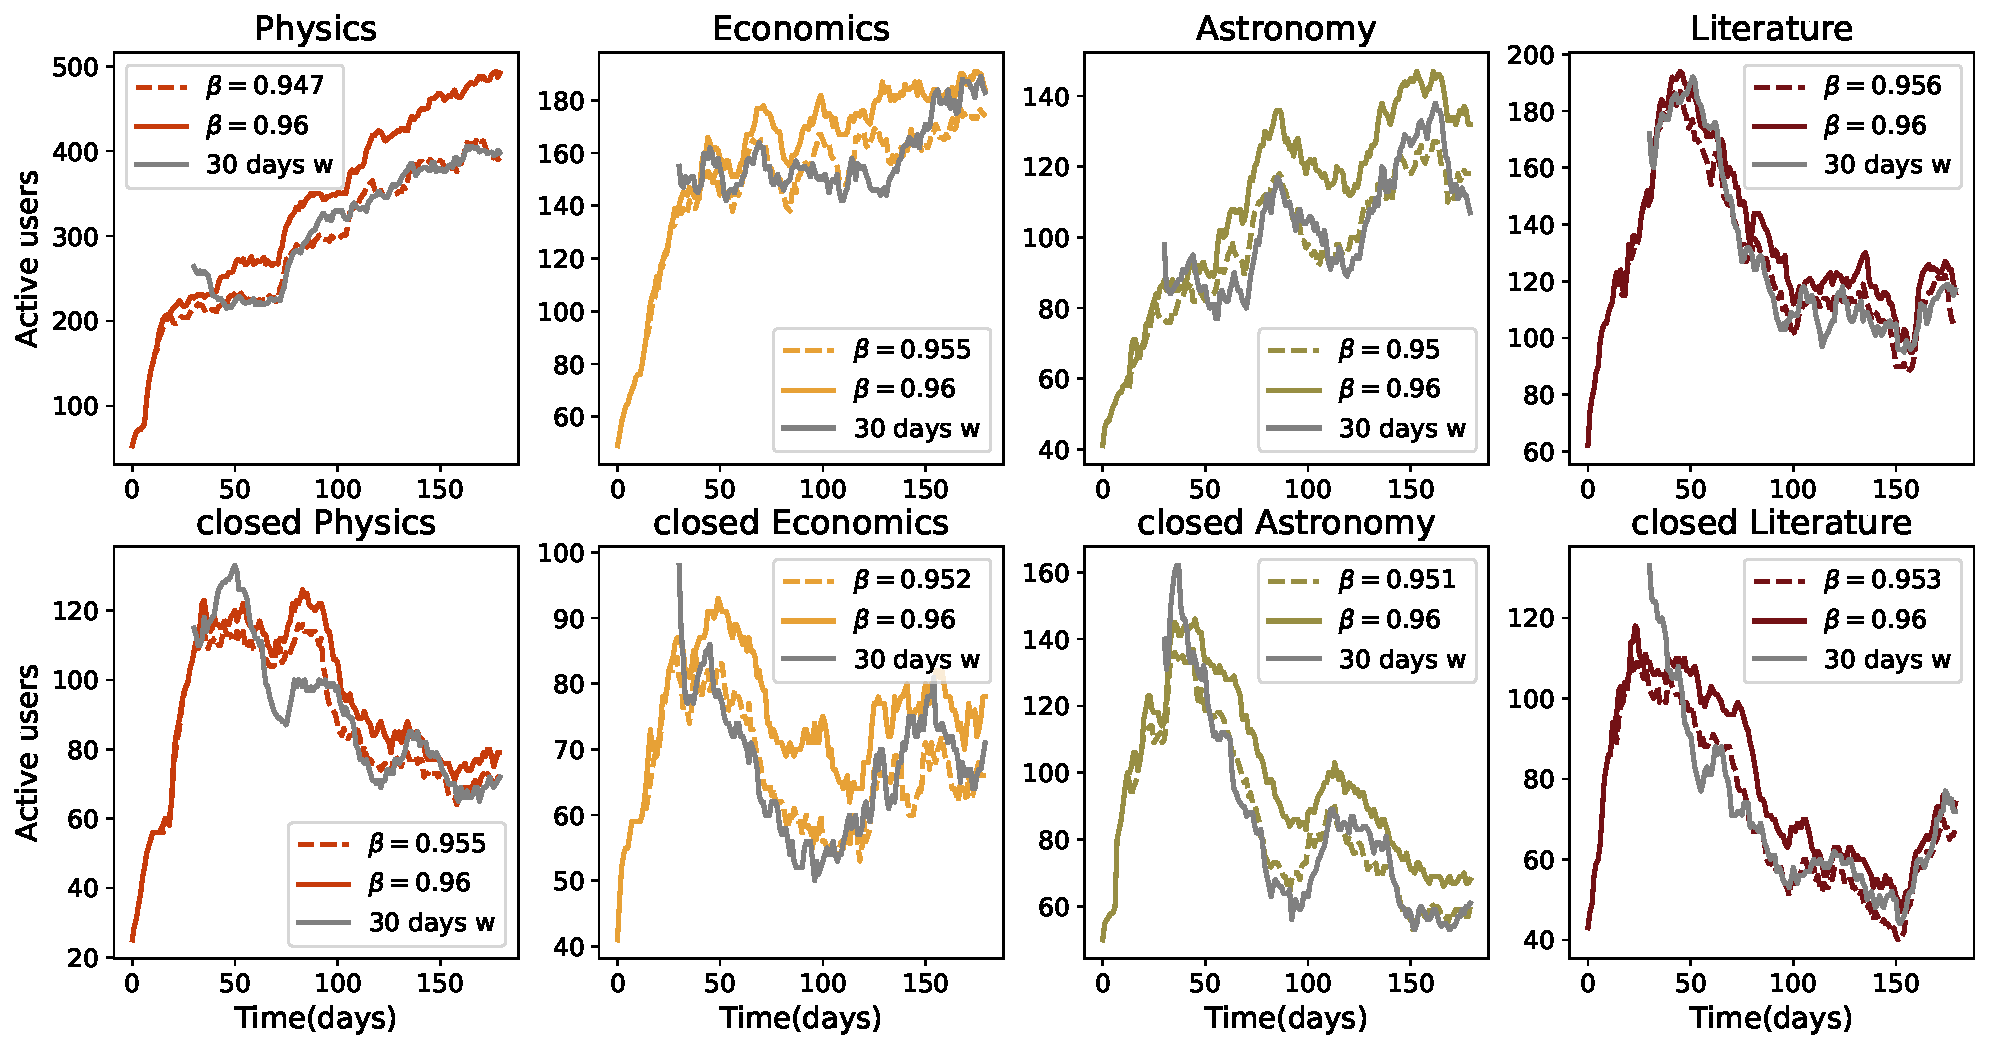
\includegraphics[width=\linewidth]{figures/stackexchange/active_users.pdf}
	\caption[Number of users in 30 days sliding window and positive reputation.]{Number of active users in a sliding window of 30 days and number of users with dynamic reputation higher than 1 for $\beta=0.954$ and $\beta=0.96 $ which provide the best fit to the number of users in 30 days sub-networks for each community}
	\label{fig:nusers}
\end{figure}

Finally, it's imporant that our dynamic reptuation captures the trend of long-term user activity. In Figure~\ref{fig:active-users} solid lines show the time series of estimated dynamic reputation for $\beta = 0.96$ while dashed lines show the number of users who were active in a given sliding window and continued to be active in the next one. Although the total estimated number of active users is expectedly higher, two time series follow similar trends in different communities.

\begin{figure}[H]
	\centering
	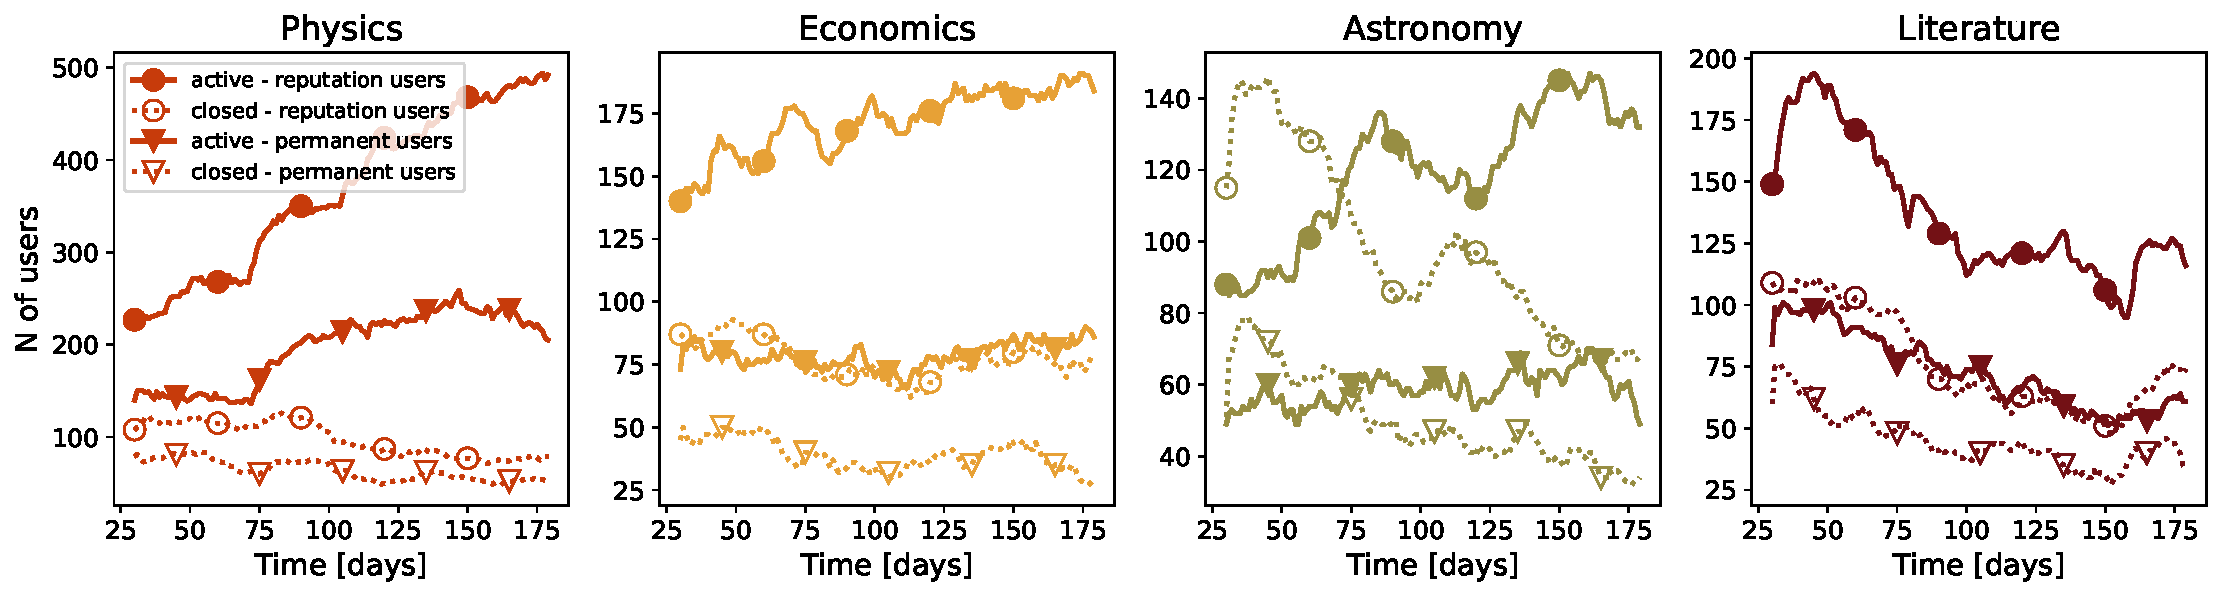
\includegraphics[width=1\linewidth]{figures/stackexchange/permanent_users.pdf}
	\caption[Number of users in Stack Exchange community who remain to be active]{Solid lines represent number of users with dynamic reputation higher than 1 for $\beta=0.96$ while dashed lines are number of users within 30 days sliding window who were active and remained to be active. Blue lines are beta, while red lines are area51 communities.}
	\label{fig:active-users}
\end{figure}

\clearpage
